\documentclass[twocolumn]{article}
\usepackage{graphicx} % Required for inserting images
\usepackage{booktabs}
\usepackage{pdflscape}
\usepackage{amsmath}
\usepackage{siunitx}
\usepackage{float}
\usepackage{url}
\usepackage{hyperref}
\usepackage[
    backend=biber,
    style=numeric
]{biblatex}
\addbibresource{Primo_BibTeX_Export.bib}
\hypersetup{
    colorlinks=true,
    linkcolor=blue,
    filecolor=magenta,      
    urlcolor=cyan,
    pdftitle={Overleaf Example},
    pdfpagemode=FullScreen,
    }
\usepackage{geometry}
\geometry{
 a4paper,
 total={170mm,257mm},
 left=20mm,
 top=20mm,
 }
\setcounter{secnumdepth}{0}
% \usepackage{float}
\title{STAT3006 A4}
\author{Avatar Azka - 47286238}
\date{November 2023}

\def\mylist#1 {\ifx!#1\else\makebox[4em][r]{#1} \expandafter\mylist\fi}
\begin{document}

\onecolumn
\maketitle
\tableofcontents

\newpage
\twocolumn
\section{Notes}
Aarøe et al. (2010) \cite{Aarøe2010} stated that the data had been standardised, however cursory examination of the data showed that the means and standard deviations of each feature did not match the expected values of standardised data (i.e. means were not equal to 0, standard deviations not equal to 1), which was odd. Thus, further Z-Score normalization was used to standardise the data. This was done in order to ensure all features are scaled similarly, such that features of different scales would not dominate (i.e. in PCA). 

\section{1. (5 Marks) PCA on Gene Expression Dataset}
Principal Component Analysis (PCA) was done on the dataset features to reduce the dimensions from 11217 genes to 121 principal components, which each represent a linear combination of the genes. 

The detailed results of each principal component's direction in terms of the original features can be found in \path{supplementary/PrincipalComponentDirections.csv}, which is a commas-separated values file where each row represents a principal component in descending order of proportion of explained variance. The first column of the file represents the index of the principal component, whereas every columns afterwards represents the coefficients of each original feature of the dataset in the linear combination that results in the principal component.

\begin{figure}[H]
    \centering
    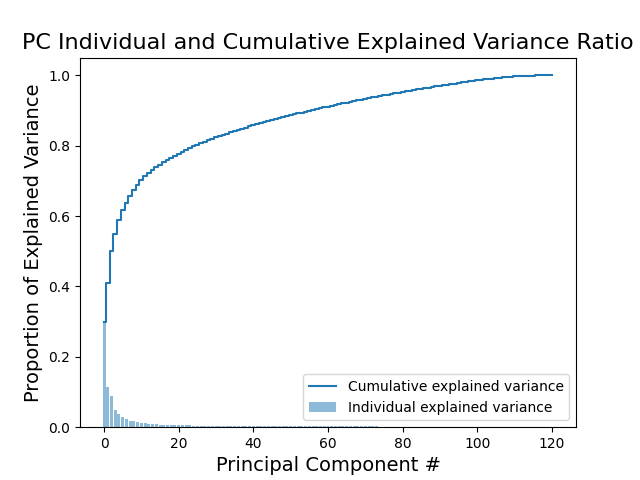
\includegraphics[width=\linewidth]{figures/PCA_Explained_Variance_Curve.png}
    \caption{Individual and cumulative proportions of variance explained by each component, sorted by descending order of explained variance ratio}
    \label{fig:pc-variance}
\end{figure}

\begin{figure}[H]
    \centering
    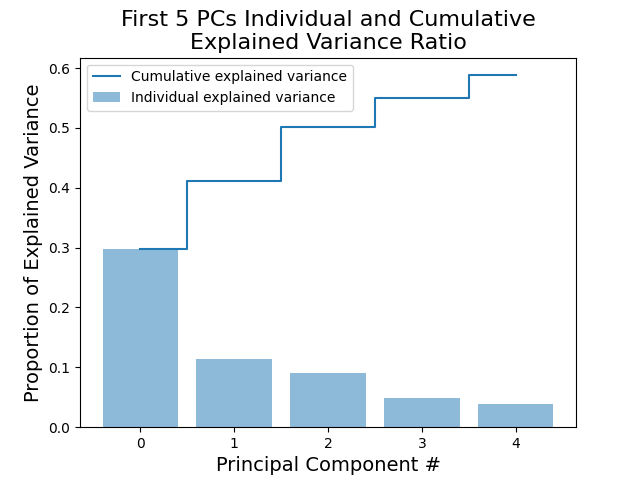
\includegraphics[width=\linewidth]{figures/PCA_Top_5_Explained_Variance_Curve.png}
    \caption{Individual and cumulative proportions of variance explained by the first 5 principal components, sorted by descending order of explained variance ratio}
    \label{fig:pc-variance-first-5}
\end{figure}


\section{2. (4 Marks) Single Variable Analysis}

\begin{figure}[H]
    \centering
    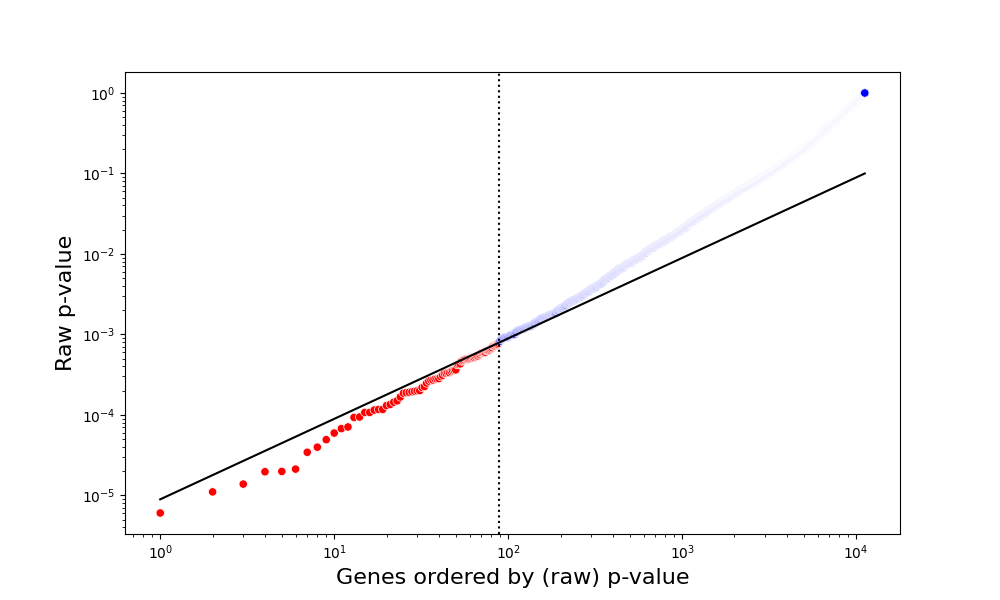
\includegraphics[width=\linewidth]{figures/SVA_Significant_Genes.png}
    \caption{Genes ordered by $p$-values $p_(j)$, and the line $0.1\cdot(j/11,217)$, representing the adjusted $p$-value threshold for the Benjamini-Hochberg method. Here the threshold lies at $j=88$, where the vertical dotted line is drawn.}
    \label{fig:bh-threshold}
\end{figure}

\section{3. (3 Marks) Defining Binary Logistic Regression With Lasso Penalty}
TODO: l1 regression etc etc

\section{4. (3 Marks) Benefits \& Drawbacks of using PCA for Dimensionality Reduction}
PCA can reduce the dimensionality of the data by transforming its explanatory variables into principal components, whose values are linear combinations of the original explanatory variables that accounts for as much of the variance in the data as possible. In the context of being able to fit this transformed data to a classifier, this comes with the benefit of 

\section{5. Classification}

The models used in this section are the Lasso-penalized Logistic Regression (henceforth LLR) and Source Vector Machine (SVM) Classifiers. 

For the LLR classifier, the regularisation hyperparameter $\lambda$ for the LLR classifier was determined via nested cross validation, as explained in section 5c.

The SVM classifier utilized a linear kernel, as informed by Hastie et al. (2009) (p.659) \cite{HastieTrevor2009EoSL}, where the authors state that while the aim of fitting nonlinear decision boundaries for SVM classifiers, such models are already sufficiently complex in cases where $p \gg N$. The regularisation hyperparameter $\lambda$ for the SVM classifier is left as the default value $1.0$. This was based on Hastie et al. (2009) (p.658) \cite{HastieTrevor2009EoSL} in which the authors state that error rates for SVM classifiers on high dimensional data are insensitive to the choice of the regularisation hyperparameter. 

\subsection{a. (1 Marks) Characterisation of Each Class}

We can make characterisations of each class by examining both the confusion matrices of each classifier, as well as the computed coefficients of each feature. Figures \ref{fig:cm-lasso} and \ref{fig:cm-svm} show the confusion matrices for the LLR and svm classifiers respectively.

\begin{figure}[H]
    \centering
    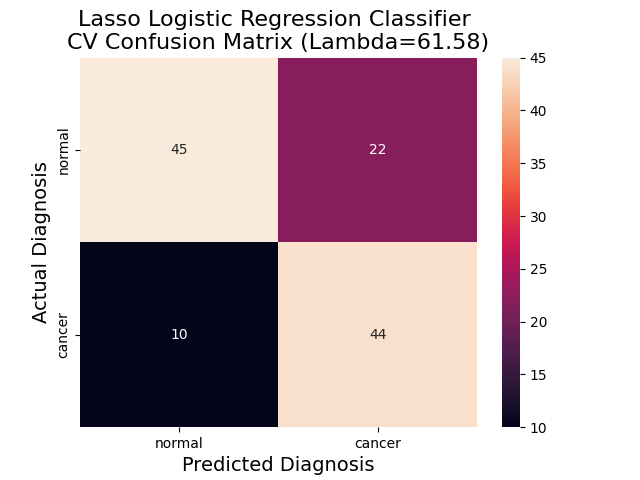
\includegraphics[width=\linewidth]{figures/Lasso_Logistic_Regression_Classifier_CV_Confusion_Matrix.png}
    \caption{Confusion matrix for the LLR classifier, estimated via 10-fold CV with $\lambda = 61.58$ (see section 5c for how this value was determined)}
    \label{fig:cm-lasso}
\end{figure}

\begin{figure}[H]
    \centering
    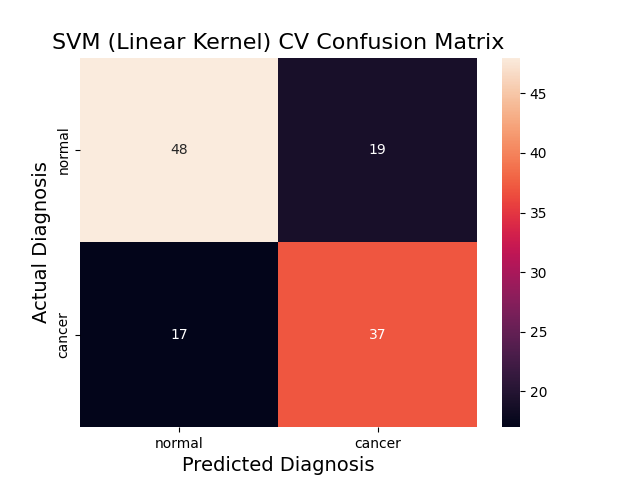
\includegraphics[width=\linewidth]{figures/SVM_(Linear_Kernel)_CV_Confusion_Matrix.png}
    \caption{Confusion matrix for the SVM classifier, estimated via 10-fold CV}
    \label{fig:cm-svm}
\end{figure}

\subsection{b. (2 Marks) CV-based Error Rate Estimates}

\subsection{c. (3 Marks) Finding The Optimal Value of Lambda}

\begin{figure}[H]
    \centering
    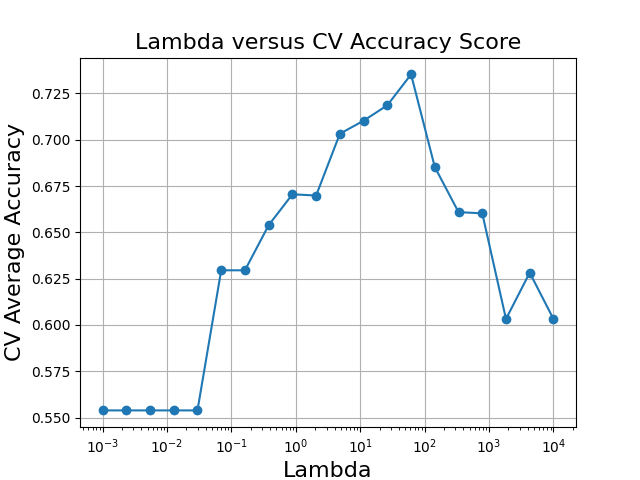
\includegraphics[width=\linewidth]{figures/Lambda_versus_CV_Accuracy_Score.png}
    \caption{Impact of the choice of the LLR regularisation hyperparameter $\lambda$ on the accuracy of the classifier. Here, the x axis is set to a log scale to reflect the search space over potential values of $\lambda$}
    \label{fig:lambda-search}
\end{figure}

\section{6. (4 Marks) Results Comparison}

Figures \ref{fig:pp-pca}, \ref{fig:pp-pca-significant}, \ref{fig:pp-lasso}, \ref{fig:pp-svm}, \ref{fig:pp-sva} in the Appendix (also available in \path{figures/PairPlot*} in the supplementary files) show plots of class distributions over pairs of features and principal components deemed significant by each analytical method. From these pair plots we can see a visual representation of how well these methods identify genes that are expressed differently between the cancer and normal groups, both individually (in each of the plots' main diagonals) and pair-wise.

Visually, it can be observed that 



\newpage
% \section{References}
\printbibliography[
    heading=bibintoc,
    title={References}
]

\newpage
\onecolumn
\section{Appendix}
\subsection{5c. Lambda Search Space}
20 potential values for $\lambda$, spread evenly between $\num{1e-3}$ to $\num{1e4}$:


\begin{table}[H]
    \centering
    \begin{tabular}{cccc}
        1.00e-03& 2.33e-03& 5.45e-03& 1.27e-02 \\
        2.97e-02& 6.95e-02& 1.62e-01& 3.79e-01 \\
        8.85e-01& 2.06e+00& 4.83e+00& 1.12e+01 \\
        2.63e+01& 6.15e+01& 1.43e+02& 3.35e+02 \\
        7.84e+02& 1.83e+03& 4.28e+03& 1.00e+04 \\
    \end{tabular}
\end{table}

\subsection{5c. Gene Importance}

\begin{table}[h!]
    \begin{tabular}{lr}
    \toprule
     & coef \\
    \midrule
    105982 & 0.567246 \\
    162796 & 0.488020 \\
    710141 & 0.470698 \\
    229944 & -0.457330 \\
    182204 & 0.449716 \\
    221030 & -0.439259 \\
    106478 & -0.439046 \\
    192905 & 0.431565 \\
    168498 & 0.412588 \\
    186433 & 0.394274 \\
    156497 & -0.390394 \\
    185593 & 0.383622 \\
    180577 & 0.380414 \\
    187446 & -0.373134 \\
    125981 & 0.372778 \\
    213145 & -0.361821 \\
    222840 & 0.357356 \\
    208243 & 0.355445 \\
    127723 & 0.353830 \\
    150701 & -0.349412 \\
    107457 & -0.339129 \\
    151002 & -0.333791 \\
    115418 & -0.331658 \\
    216357 & -0.304303 \\
    243149 & -0.302698 \\
    196441 & -0.299391 \\
    180804 & 0.292722 \\
    203708 & 0.289368 \\
    203664 & 0.288367 \\
    104116 & 0.282697 \\
    \bottomrule
    \end{tabular}
\end{table}

\subsection{6. Class Distribution Pair Plots}
\begin{figure}[H]
    \centering
    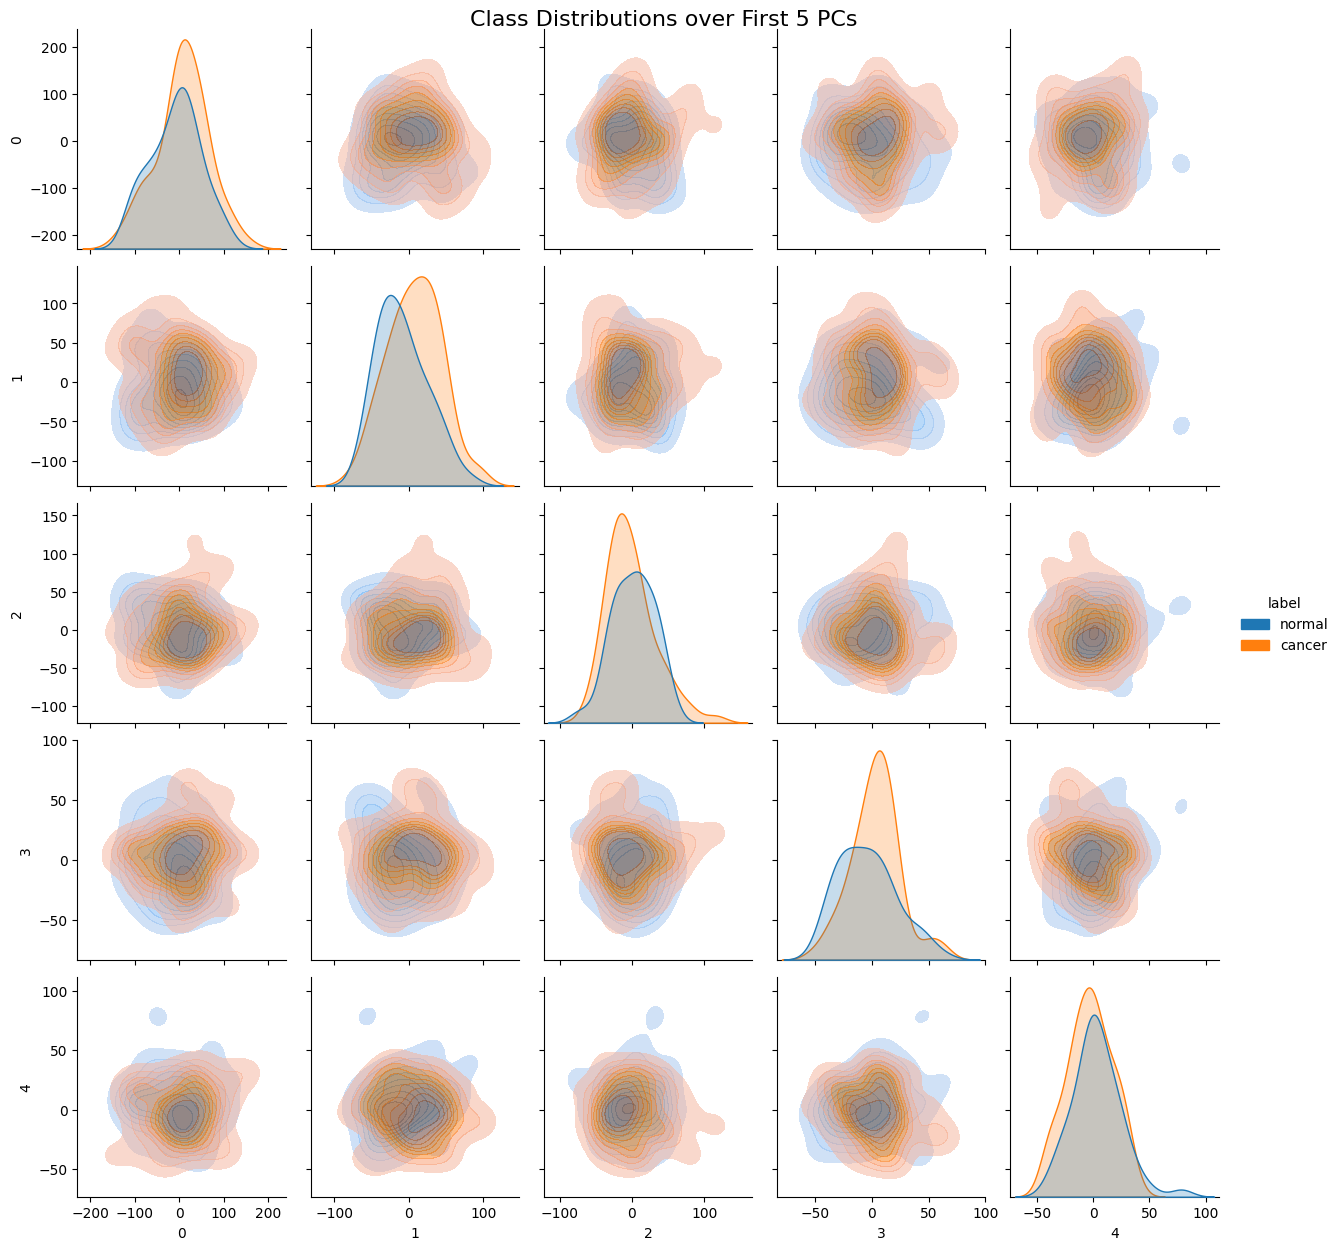
\includegraphics[width=0.85\linewidth]{figures/PairPlot_PCA.png}
    \caption{Pair plot of class distributions over the first 5 principal components in order of explained variance ratio}
    \label{fig:pp-pca}
\end{figure}

\begin{figure}[H]
    \centering
    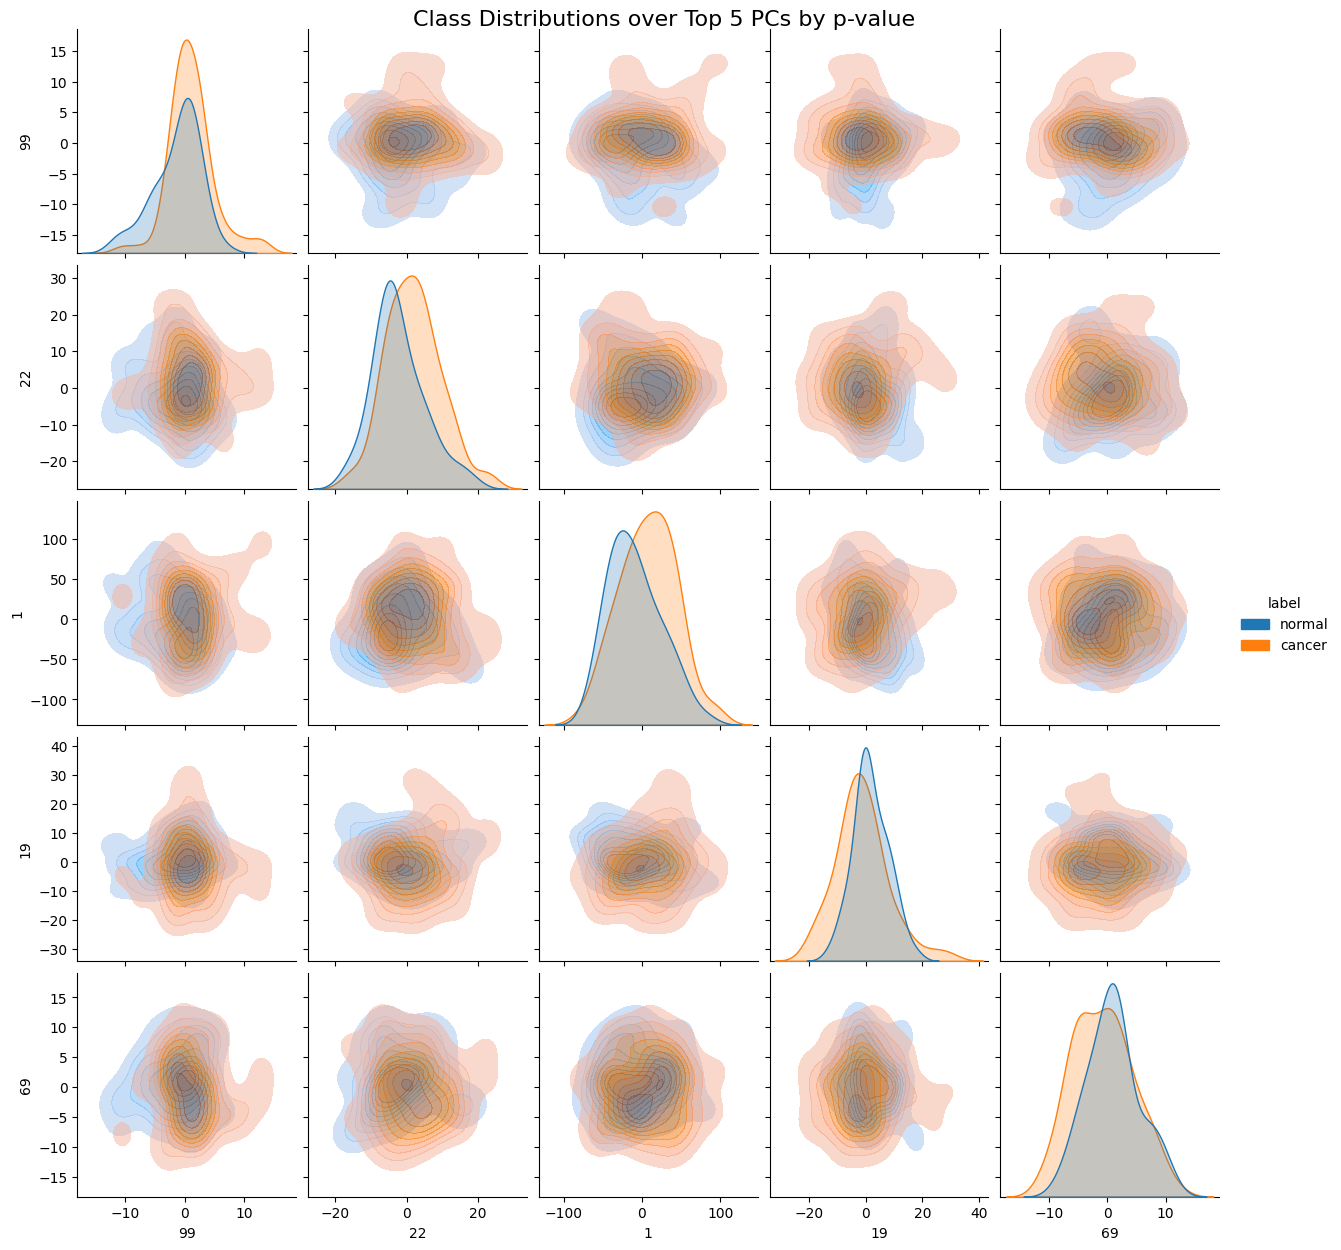
\includegraphics[width=0.85\linewidth]{figures/PairPlot_PCA_Significant.png}
    \caption{Pair plot of class distributions over the top 5 principal components in order of p-value}
    \label{fig:pp-pca-significant}
\end{figure}

\begin{figure}[H]
    \centering
    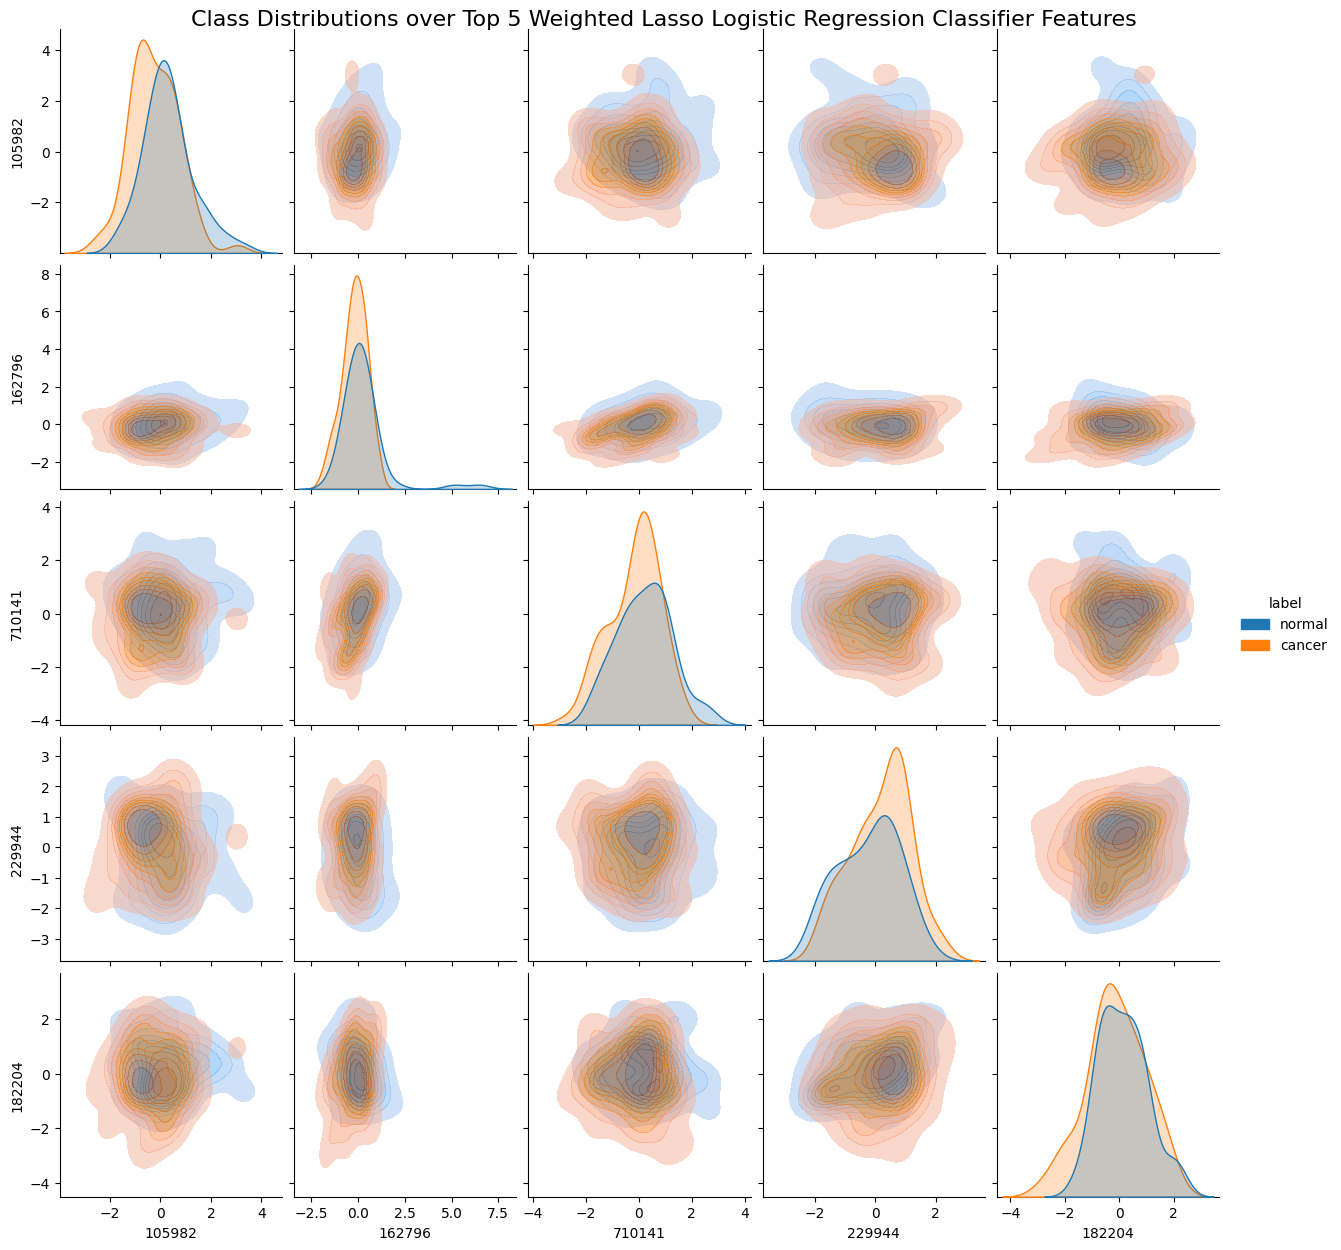
\includegraphics[width=0.85\linewidth]{figures/PairPlot_Lasso.png}
    \caption{Pair plot of class distributions over the top 5 weighted features in the LLR classifier}
    \label{fig:pp-lasso}
\end{figure}

\begin{figure}[H]
    \centering
    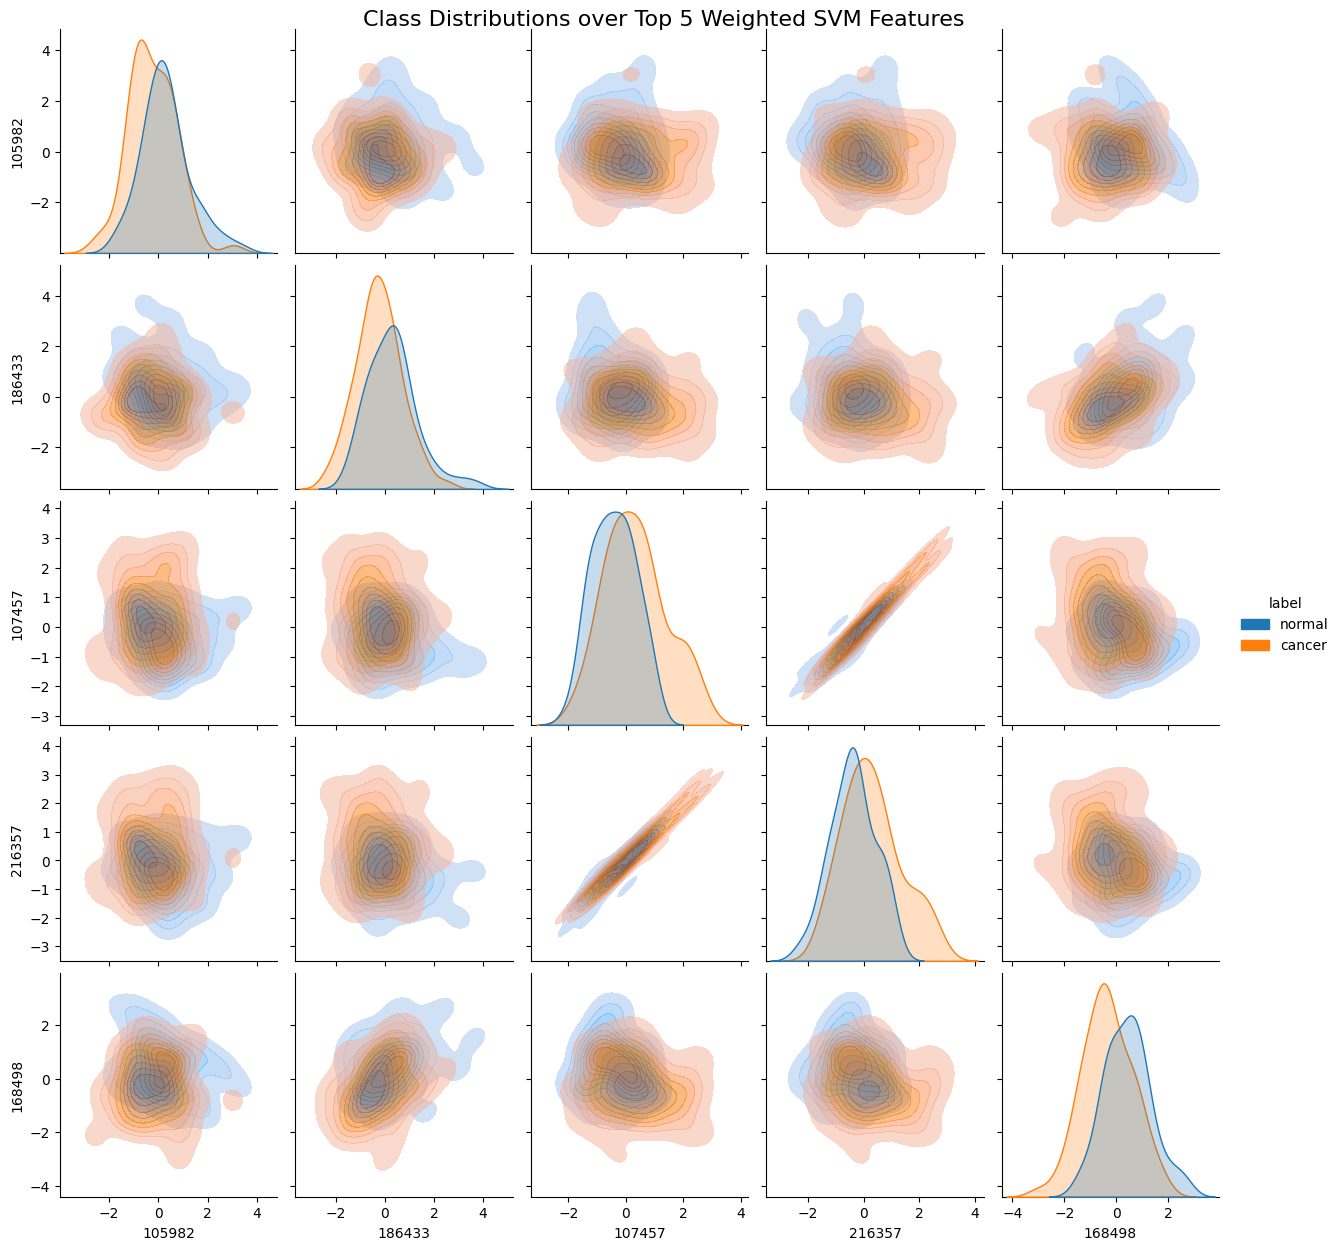
\includegraphics[width=0.85\linewidth]{figures/PairPlot_SVM.png}
    \caption{Pair plot of class distributions over the top 5 weighted features in the SVM classifier}
    \label{fig:pp-svm}
\end{figure}

\begin{figure}[H]
    \centering
    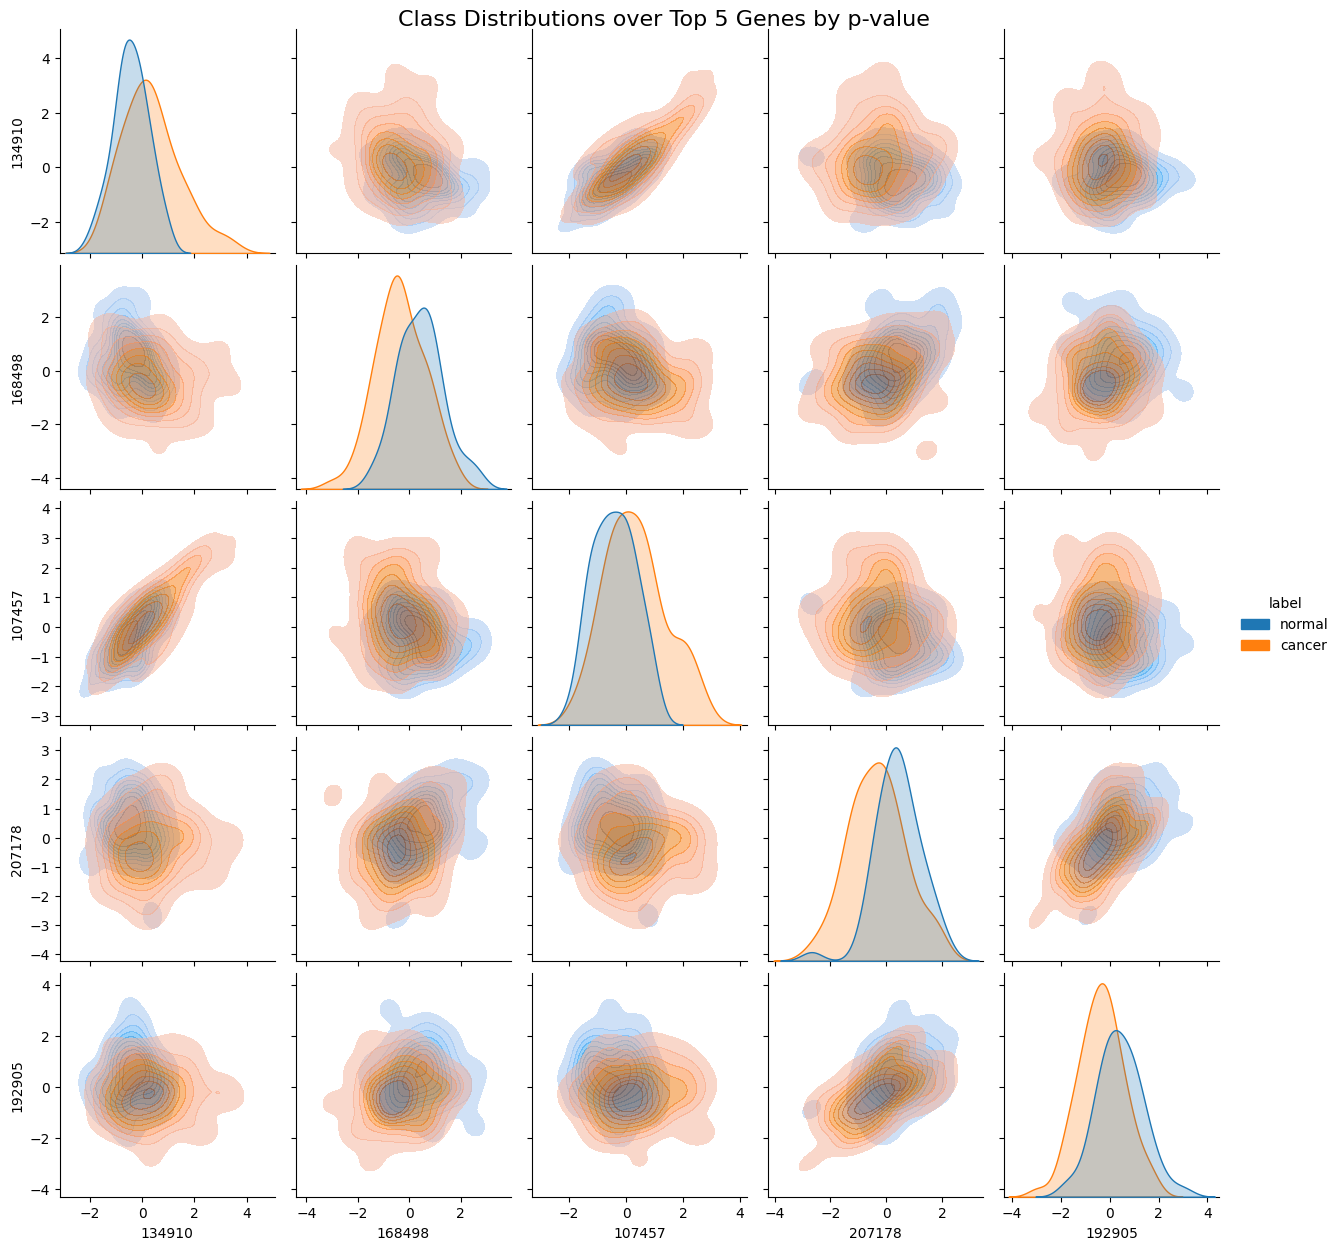
\includegraphics[width=0.85\linewidth]{figures/PairPlot_SVA.png}
    \caption{Pair plot of class distributions over the top 5 significant features based on p-value}
    \label{fig:pp-sva}
\end{figure}

\end{document}